\chapter{背侧前额叶皮层:基于最近事件生成目标} \label{chap:chap6}
背侧PF皮层有助于根据顺序、时间和空间环境生成目标,它的连接解释了为什么只有它才能做到这一点。背侧PF皮层,包括中外侧PF皮层(46区),通过与后顶叶皮层、前运动皮层和PF皮层的其他部分连接来发挥作用。顶叶连接提供了许多用于生成目标的空间和时间背景。与运动前区域的联系导致这些目标的实现,通常是通过手的运动。与眶侧PF皮层的连接使背侧PF皮层能够根据单个事件预测目标选择的具体结果。背侧PF皮层位于背侧视觉流的末端,因此它可以规划目标序列,它可以具体或抽象地指定这些目标。在产生目标后,背侧PF皮层可以前瞻性地编码它们,直到行动的时候到来。鉴于背侧PF皮层在类人猿灵长类动物中进化(第2章),我们认为它在使用最近视觉事件的顺序、时间和位置来指导觅食选择和生成效率优化的目标序列方面具有优势。

\section{介绍}
第二章解释了灵长类动物的PF皮层在类人猿中随着新区域的出现而扩展。第三章涉及了其中的一些,例如极性PF皮层(10区),但在本章和下一章,它们是主要主题。由于类人猿依赖于白天漫长的觅食旅行,它们需要消耗大量的能量,并面临着很高的捕食风险。这种生活方式非常重视正确的觅食选择。在影响这种选择的因素中,视觉事件的位置、时间和顺序是突出的,因为类人猿利用了它们在中央凹和色彩视觉方面的进步。正如第二章所解释的,这些进步包括中央凹提供的精致的视觉敏锐度和三色视觉提供的增强的辨别能力。

这一章解释了觅食的选择部分取决于当前的环境,这是由选择时可用的刺激以及最近视觉事件的记忆所指定的。为了理解我们的意思,考虑一个简单的实验室任务:延迟匹配样本。猴子把一个刺激看作一个样本,然后看到一个或多个刺激需要选择。这种选择不仅取决于选择时的刺激,还取决于基于样本刺激的记忆。这两个因素共同构成了当前选择目标的背景。

由于记忆对当前情境起作用,这类实验的被试面临一个问题:最近发生了几件事,并选择了几个目标。本章的大部分内容探讨了背侧PF皮层如何帮助类人猿灵长类动物解决这个问题。许多文献都依赖于一个任务和一个区域:延迟反应任务,它依赖于中外侧PF皮层(46区)。因此,我们将讨论的重点放在第一章和第五章也提到的这个任务上。我们认为,因为受试者在这个任务中经历了一系列的视觉事件,并实现了一系列的目标,他们需要挑选出决定当前目标的事件。然后,我们回顾一系列其他任务,这些任务也要求主体在当前环境的基础上生成目标。
\section{区域}
在猕猴中,中外侧PF皮层位于主枕沟的吻侧三分之二(图6.1)。然而,它也延伸到这个沟的背侧和腹侧的凸面皮层。中外侧PF皮层(46区)有很多名字,有些很明确,有些则不太明确。
\begin{figure}
	\centering
	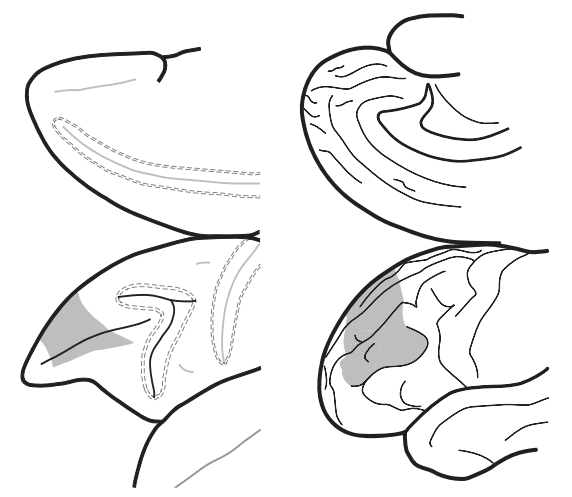
\includegraphics[width=0.7\linewidth]{image_pfc/Fig_6_1}
	\caption{猕猴(左)和人类(右)的背侧PF皮层。格式如图1.2所示。}
	\label{fig:fig}
\end{figure}

Walker(1940)将沿主沟整个长度的皮层称为46区,但最近Petrides和Pandya(1999)将9/46区区分为该沟的尾端周围(见图1.2)。为了避免对46这个术语的不同用法的混淆,我们称沃克46区吻侧三分之二为中外侧PF皮层,尾侧三分之一为后外侧PF皮层。在人类中,这些分区位于额上回和额下沟之间。

尽管出现了这些新术语,但混淆的空间仍然很大。术语背侧前额叶皮层最初是指猴子的整个侧前额叶皮层(Pribram et al. 1952),但后来仅指主沟内和背侧的皮层(Mishkin et al. 1969)。在影像学文献中,指PF背外侧皮层已变得很常见,但该术语的使用通常非常松散,很少注意解剖标志。因此,我们在本书中避免使用这个术语。表1.2给出了我们所采用的术语。我们将PF背侧皮层包括主沟两岸的皮层和其背侧的凸面皮层(区域9),但不包括区域9的内侧部分。当然,这些划分并不是最终的结果,但它们在一定程度上反映了联系。
\section{连接}
图6.2展示了PF皮层背侧的一些皮质连接。正如第一章所解释的,这些连接构成了解剖指纹。
\par
1.中外侧PF皮层(46区)与后顶叶皮层,特别是尾顶叶区有很强的联系(Petrides \& Pandya 1984,1999,2009)。正如前一章所提到的,后顶叶皮层的许多神经元编码视觉空间信息。然而,顶叶细胞也编码时间间隔(Leon \& Shadlen 2003),当人类受试者对近期事件做出判断时,左侧顶叶内沟会出现激活(Dudukovic \& Wagner 2007)。
\par
2.中外侧PF皮层连同外侧9区,与位于颞上沟上岸的多模态区TPO区(也称为颞上多感觉区STP)相连(Seltzer et al. 1996;Petrides \& Pandya1999)。该区域的细胞对体感、听觉和视觉刺激有反应(Bruce et al. 1981)。
\par
3.中外侧PF皮层也接受来自周围皮层的输入(Petrides \& Pandya 1999),其功能是识别物体(Murray et al. 2007)。这种联系表明,中外侧前额叶皮层接收到有关物体的直接输入,而不仅仅是腹侧前额叶皮层的间接输入(第7章和第8章)。
\par
4.中外侧前额叶皮层接收来自次级体感觉区(S2) (Petrides \& Pandya 2002b)和下颞叶皮层吻侧PFG区(Rozzi etal . 2006)的输入。这些区域的细胞对体感刺激有反应(Hyvarinen 1981),中外侧PF皮层的细胞也是如此(Tanila et al. 1993)。这一特征将中外侧PF皮层与尾侧和后外侧PF皮层区分开来,后者的细胞主要具有视觉和注意力特性(第5章)。
\par
5.中外侧PF皮层连接背侧和腹侧前运动皮层(Wang et al. 2002),以及前辅助运动区(preSMA) (Wang et al. 2005)和位于扣带沟的扣带吻侧运动区(CMAr) (Dum \& Strick 1993)。这些投影主要涉及代表手和手臂的运动前区域,而不是脚和腿。前肢表征的专门化表现在背侧前前皮层的吻侧部分(Tachibana et al. 2004)、腹侧前运动皮层(He et al. 1993)、preSMA (Luppino et al. 1991)和CMAr (He et al. 1995)。因此,相对于运动的运动,中外侧PF皮层在伸手、操作和进食运动中具有优先的作用(第2章)。
\par
6.中外侧PF皮层与前扣带皮层有很强的联系(Petrides \& Pandya 1999)。第3章解释了前扣带皮层在动作的评估和基于这些评估的动作之间的切换中发挥作用(Walton et al. 2007)。
\par
7.中外侧PF皮层与脾后皮层相连(Morris et al. 1999)。反过来,从脾后皮层投射到海马旁回和下丘前(Kobayashi \& Amaral 2007)。我们认为,这些联系可能在有关事件的记忆检索中发挥作用,而这种检索依赖于时间或空间上下文(Vann et al. 2009)。
\par
8.区域9的横向部分的连接受到的关注相对较少,部分原因是很少有功能数据引起人们的兴趣。这部分背侧PF皮层与背侧运动前皮层的吻侧部分(Petrides \& Pandya 1999)和CMAr (Morecraft \& van Hoesen 1993)有联系。就像第9区域的内侧部分一样,它也与上颞皮质有联系,这可能传达听觉信息(Petrides \& Pandya 1984;Saleem et al. 2008)。最后,第9区外侧部分与后顶叶皮层下部(PG区)(Cavada \& Goldman-Rakic 1989)和脾后皮层(Kobayashi \& Amaral 2003)相连。
\begin{figure}
	\centering
	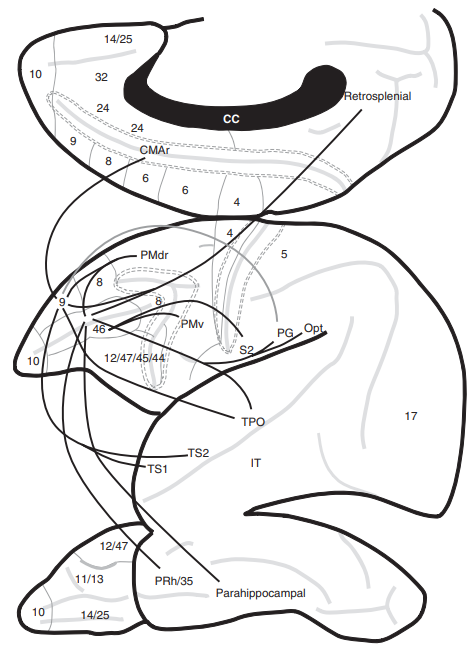
\includegraphics[width=0.5\linewidth]{image_pfc/Fig_6_2}
	\caption{PF皮层背侧的选定连接。图1.4和1.5给出了沟和区域的名称。一些轴突与背侧PF皮层有直接连接的区域被认为是相互的,除非另有说明。}
	\label{fig:fig}
\end{figure}

\subsection{总结}
中外侧PF皮层与后顶叶皮层、前运动皮层有很强的联系,并间接与海马系统有联系。它也与PF皮层的其他部分相互连接,如眶PF皮层。其他皮质区域没有这种连接模式。因此,它很好地整合了由眶前PF皮层、背侧视觉流和海马体处理的信息,并向运动前皮层提供信息。

\section{延迟响应任务}
中外侧前额叶皮层在接收后顶叶皮层的视觉空间信息方面与尾侧前额叶皮层相似。因此,任何一个区域的损伤都会导致猴子在动眼延迟反应任务和经典版本的延迟反应任务上的表现中断,这并不奇怪。在这两项任务中,空间线索指导目标选择,猴子必须在可能的空间目标中进行选择。当然,根据定义,动眼肌延迟反应任务需要对目标进行扫视,而经典的延迟反应任务需要达到目标的运动。第5章解释了尾侧PF皮层和后外侧PF皮层的损伤会导致动眼力延迟反应任务的准确性误差,根据它们与背侧视觉流的连接,这是有意义的。这些损伤不会引起很多明显的错误,当它们发生时,猴子会迅速纠正这些错误(Tsujimoto \& Postle 2012)。

相反,中外侧PF皮层(46区)的永久性损伤对经典的延迟反应任务造成毁灭性的损害。当猴子在手术前学习延迟反应任务时,它们在中外侧PF皮层损伤后执行任务的效果并不比偶然水平好(Goldman \& Galkin 1978)。也就是说,受损的猴子犯的错误和正确的选择一样多。当他们在中外侧PF皮层持续受损后第一次尝试学习任务时,即使有短暂的(1秒)延迟期,他们也无法完成任务(Battig et al. 1960)。而且它们永远无法恢复,至少在任何人测试过的时间范围内都无法恢复。

一个重要的方法差异可以解释这种差异的部分原因。在经典的延迟反应任务中,猴子伸手去拿盖在食物井上的盖子。这意味着在这个版本的任务中,不像动眼肌延迟反应任务,受试者只能犯明显的错误。精度错误,如果发生,将不会被记录。

另一个区别可能也很重要。猴子可以通过在延迟期间偷偷地关注目标位置来解决动眼肌延迟反应任务。但是实验者执行经典延迟反应任务的方式使得隐蔽注意力很难集中到目标上。传统的测试方法包括威斯康星通用测试装置(WGTA)。在该装置中,一个不透明的屏幕在延迟期间下降,使猴子在延迟期间无法看到相关位置(图6.3)。在神眼运动版本的任务中,猴子可以在周边视觉中看到目标位置,尽管在扫视时它不再被标记出来。

原则上,执行经典延迟反应任务的猴子仍然可以准确地注意到WGTA的目标一侧,或者以某种方式将姿势定向到那一侧。然而,降低屏幕往往会导致猴子在测试室内移动。Passingham(1971)在延迟期间监测了正常猴子的位置,发现即使它们已经解决了问题,在40\%的试验中,它们也会从房间的一边穿过到另一边。因此,猕猴不需要通过身体定位来解决延迟反应任务所带来的问题,似乎测试方法很可能排除了使用隐蔽注意力来解决这个问题。因此,动眼肌延迟反应相对缺乏坦率的错误可能反映了隐蔽地关注目标位置的持续能力,而延迟反应任务的经典版本的严重损害可能是由于破坏了这一策略。

当然,延迟响应任务可以在没有不透明屏幕的情况下呈现。在延迟期间,食物井可能在受试者够不到的地方。在这种情况下,猴子似乎更有可能采取某种姿势或注意力的方法来弥合延迟期,或者使用其他策略来做到这一点。Wilson et al.(1963)发现。正常的猴子在延迟期开始时坐在测试室的正确一侧,在延迟期结束时仍保持在该一侧。然后,当他们有机会这样做时,他们就会到达离目标最近的距离。在延迟开始时,有PF皮层损伤的猴子也坐在正确的一侧,但在延迟结束时,它们到达相反(错误的)目标的次数与到达正确目标的距离较短的次数一样多。这一发现表明,对于有PF损伤的猴子来说,姿势或注意力的延迟期桥接不足以正确地形成延迟反应任务。

目前还不清楚为什么猴子在整个延迟期间不采取保持在WGTA正确一侧的策略。这个策略可以解决问题。也许他们没有意识到,他们在延迟期开始时看到的东西表明了他们在延迟期结束时应该达到的目标。换句话说,受损的猴子可能无法识别延迟间隔之前的视觉事件与它们即将做出的选择有任何关联。正常的猴子确实认识到这种关系,并且不需要采取姿势定向策略或注意力策略来执行任务。

在后面的部分中,我们提出了这样的想法,即为了解决延迟响应任务所带来的问题,猴子需要知道延迟期之前的视觉事件为它们之后选择目标提供了关键。我们认为,中外侧前额叶皮层受损的猴子要么无法学习这一规则,要么无法记住和应用它。

\begin{figure}
	\centering
	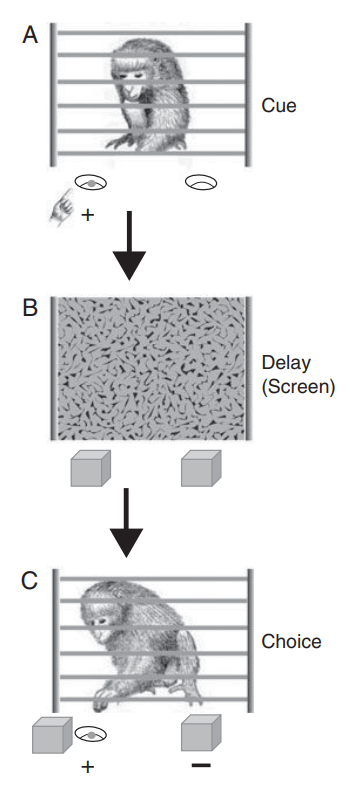
\includegraphics[width=0.2\linewidth]{image_pfc/Fig_6_3}
	\caption{在威斯康星州通用测试装置(WGTA)中延迟响应任务的测试程序。(A)实验员在两个食物井(+)中的一个上饵,一只猴子从它的测试笼中观察。这个动作作为视觉提示事件。(B)实验者在延迟期间放下一个不透明的屏幕。相同的物体可以很好地覆盖食物。(C)实验者举起屏幕后,猴子在两个食物井中进行选择,将其中一个物体移开,如果正确(+)则获得奖励,如果错误(-)则得不到奖励。修改自Murray EA.杏仁核复合体对猕猴行为的贡献。脑研究进展87:167-80©1991,Elsevier许可。}
	\label{fig:fig}
\end{figure}
\subsection{延迟期的重要性}
第5章提到,尽管尾侧PF皮层病变的猴子在动眼力延迟反应任务上只有轻微的损伤,但它们在没有延迟期的条状视动任务上也有损伤。相比之下,在中外侧前额叶皮层有损伤的猴子只在包括延迟期的任务中有损伤。

Passingham (1985a)设计了一个没有延迟的条件视觉运动任务。显示器中央的两个面板,一个在另一个上面,提供线索。猴子们知道,如果光出现在顶部的面板上,那么它应该选择一侧的目标;如果一个光出现在底部面板,那么它应该选择另一边的目标。所以这个任务包括空间线索和空间目标就像延迟反应任务一样,但不像延迟反应任务它不包括延迟期。中外侧和后外侧PF皮层病变的猴子可以正常学习这项任务。

Stamm(1969)的结果也表明,延迟是产生损伤的关键因素。在一个试验中,他在不同的时间点灭活了中外侧或后外侧前额叶皮层。在延迟期的早期,中外侧PF皮层(46区)的破坏估计导致延迟反应任务的表现下降到机会水平。刺激后外侧皮层效果较小。这一发现与巴特斯(Butters)和潘迪亚(pandya)(1969)的一项研究结果一致,他们在该研究中表明,主沟中央三分之一的病变导致延迟交替任务的严重损害,而后三分之一的病变的影响要小得多。

综合来看,这些结果支持两个结论。首先,延迟响应任务的损害确实是由于延迟期的强加造成的。其次,中外侧PF皮层在这一任务中起着必要的作用。在密切相关的延迟交替任务中也是如此。
\subsection{延迟周期活动}
关于延迟反应障碍,最常被引用的说法是猴子无法记住线索的位置,因此这种缺陷可以被描述为回溯性空间工作记忆的缺陷之一。人们可以记录下延迟期间的活动,而且乍一看,这种活动似乎是对线索位置的记忆编码,这一事实被解释为支持这一结论的证据。然而,这种活动发生在PF皮层的许多部分,以及其他区域。第五章解释了延迟期活动并不总是编码空间记忆。当研究人员在充分的比较条件下研究细胞活动时,他们可以看到大部分所谓的记忆活动实际上编码了参与的位置。然而,一些延迟期活动确实编码了记忆的位置,因此,中外侧PF皮层的延迟期活动仍然有可能介导回溯性工作记忆。

Kojima和Goldman-Rakic(1984)从中外侧PF皮层(46区)进行记录,试图验证空间工作记忆理论。他们使用了两种条件。在一种情况下,线索在延迟期间消失,而在另一种情况下,线索在整个试验过程中仍然可见。在延迟期间编码位置的62个细胞中,当刺激仍然可见时,44个细胞表现出相同或更大的延迟期活动。当刺激消失时,只有12个细胞更活跃。Tsujimoto和Sawaguchi (2004b)在类似条件下使用了动眼肌延迟反应任务,并证实了这一结果模式。

对这一发现最有可能的解释有四种:
\par
1.即使线索仍然可见,也没有什么能阻止猴子“记住”它的位置。因此,在这两种情况下,它们可能会“记住”提示的位置。
\par
2.在这两种情况下,猴子可能会盯住目标。Kojima和Goldman-Rakic(1984)没有记录眼睛的位置,所以我们不能排除他们的结果是由于明显的注意力。
\par
3.在这两种情况下,猴子可能会偷偷地关注目标。
\par
4. 在这两种情况下,猴子可能会对空间目标的位置进行编码。这种表述可能包括一个计划好的行动,也可能独立于实现目标所需的行动而指定目标。

在这四种解释中,只有第一种与Kojima和Goldman-Rakic(1984)的解释是一致的。他们得出的结论是,延迟期的活动反映了线索在回顾记忆中的位置,这与空间工作记忆理论一致。然而,猴子似乎不太可能“记住”它们能看到的刺激。第二种说法,就公开关注而言,可以解释小岛和戈曼-拉基奇的结果,但不能解释辻本和泽口的结果。在后一项研究中,猴子必须在整个延迟期间固定在一个中心位置。第三种解释,即隐性注意,也可以解释两项研究的结果,但它与回溯性工作记忆方面的解释不相容。

这就剩下了第四种解释,它将延迟期活动解释为反映了空间目标的位置,这是Fuster(1973)首次提出的。换句话说,这表明延迟期反映的是前瞻性记忆,而不是回顾性记忆。猴子每天进行多次试验,这意味着先前试验的线索和目标位置在记忆中相互干扰。在任何特定的试验中,只要看到线索,猴子就能通过编码目标位置来克服这种干扰。

第五章回顾了一些似乎反对目标的前瞻性编码的证据。大多数细胞编码反眼跳任务中的线索位置,只有少数编码目标位置。在另一项研究中,细胞对提示位置进行编码,即使这些位置不是未来的目标。然而,这些研究都没有明确地关注中外侧PF皮层的细胞,而不是后外侧或尾侧PF皮层。

在本章稍后将详细介绍的一项研究中,Genovesio等人(2006a)确实研究了中外侧PF皮层中的细胞,以及其他神经元种群,他们的实验设计允许他们区分位置的回顾性编码和前瞻性编码。他们发现,中外侧前额叶皮层的细胞尽可能快地编码当前的目标位置,并且回溯编码在这个时候消失。我们还在后面的一节中提供数据,表明这种预期的活跃度可以防止内存干扰(Sakai et al. 2002a)。

\subsection{总结}
中外侧PF皮层损伤的猴子在机会水平上执行延迟反应任务,并且它们没有恢复。在延迟期间的破坏性电刺激会导致损伤,在没有延迟期的任务中,猴子表现正常。延迟期活动发生在中外侧PF皮层,它编码一个位置。这种活动已经被解释为回顾性空间记忆,但证据表明,这种活动也编码了当前目标的位置(预期编码)和参与的位置。

\section{干扰的作用}
在延迟反应和延迟交替任务上,每天都有一系列的试验展开,这对记忆造成了严重的干扰。在延迟反应任务中,随着试验次数的增加,猴子会从两个或多个位置获得线索;在延迟反应和延迟交替任务中,猴子在一系列试验中选择了相同的地点。

\subsection{干扰效应的证据}
Diamond和Goldman-Rakic(1989)的一项实验表明,干扰可能是导致延迟反应障碍的重要因素。他们在修改后的延迟反应任务中测试了背侧PF损伤的猴子,并分析了猴子在两次正确选择同一侧后所犯的错误。当这次测试的正确位置碰巧与前两次测试的正确位置相匹配时,猴子的正确率为85\%。当当前试验中的正确位置与前两次试验不匹配时,猴子的表现符合概率水平(50\%正确)。

有人可能会试图解释这一发现,认为猴子坚持不懈。但是,坚持不懈会导致低于机会的表现,相反,猴子表现在机会水平(50\%正确)。事实上,受损的猴子在机会水平上的表现表明,它们意识到线索与前两次试验不同。然而,他们不知道该选择哪个位置,所以他们的选择基于这样一个事实:两种可能的选择产生的奖励频率与最近几次试验的平均值大致相同。

正常的猴子可以学会根据单一事件做出选择。在经典的延迟反应任务中,这个事件包括看到一颗花生被放在其中一个食物井里。在其他版本的延迟响应任务中,相关事件由空间某处闪烁的视觉提示组成。

在第4章中,我们指出,患有眶PF损伤的猴子不会坚持,而是根据过去的事件历史(经过多次试验的平均值)来选择对象。相比之下,完整的猴子可以将结果分配给似乎导致结果的单一、具体的选择。我们认为中外侧PF皮层也有类似的情况。在延迟响应任务中,在延迟期间之前的可视事件导致基于该单个事件生成适当的目标。如果没有这种影响,我们的选择将取决于许多先前事件的平均值。

Diamond和Goldman-Rakic使用的延迟反应任务是对Piaget(1954)设计的任务的修改,该任务用于评估人类婴儿理解物体持久性的能力。它被称为“A-not-B”任务。实验者在a位置藏了一个玩具,婴儿拿了出来。然后他们把玩具藏在位置b。即使婴儿看到这个视觉事件,他们倾向于回到位置A (Harris 1989)。

A-not-B任务通常要求婴儿伸手去找他们看不到的目标。 值得注意的是,他们有时甚至可以在透明覆盖物下看到位于B位置的物体时到达A(Butterworth 1977)。 因此,婴儿似乎记得他们在最近的过去选择了A位置来获得玩具,所以他们再次这样做,而不是根据最近的视觉事件来选择玩具。 换句话说,他们似乎重复一个最近强化的选择,而不是根据玩具隐藏在B位置的视觉事件做出选择。当儿童更成熟时,他们很容易学会使用最近的事件,即玩具隐藏在B位置,来选择那个位置作为他们的目标。

以同样的方式来看,延迟响应任务的损害可以说是解决试验间干扰的困难,而不是追溯记忆的失败。从这个角度来看,试验对试验的干扰是由先前在A-非B任务中选择位置A或先前在延迟响应任务中选择替代位置引起的。

为了支持这一想法,有影像学证据表明,当记忆受到干扰时,中外侧PF皮层的作用。Owen等人 (1999) 给人类受试者两个空间任务。在其中一个位置中,他们介绍了五个位置,并随后立即测试了这些物品的内存。另一个任务是n -back任务。在两背任务中,实验者在一系列位置呈现刺激事件,受试者必须指向两个事件之前出现刺激的位置。因此,n -back任务类似于延迟响应任务,因为出现了一系列项目,并且主题必须将相关项目与无关项目区分开。空间刺激的顺序决定了相关的位置。在第一个任务中,尾部PF皮层 (区域8) 发生了激活,其顺序无关紧要,但中外侧PF皮层未发生激活。但是,在与顺序相关的n -back任务中,激活也发生在外侧PF皮层中。

Gray等人 (2003) 直接表明n -back任务涉及干扰。他们对faces使用了三背任务,并比较了高干扰和低干扰条件。高干扰条件在所有刺激演示中都使用了相同的面孔。低干扰条件使用了新颖的面孔两次或四次试验作为干扰因素。与分散注意力的面孔是新颖的相比,当分散注意力的面孔与目标面孔来自同一组时,受试者的表现要差得多。在同一项研究中,Gray等人发现,在高干扰条件下表现更好的受试者中,PF皮质中部和其他区域的激活更多。

\subsection{间隔试验}
与Gray等人 (2003) 的成像研究一样,人们可以通过直接操纵干扰来研究干扰。例如,每天只能在一次试验中测试一下猴子。Wilson等人 (1963) 做了该实验,发现即使没有试验到试验的干扰,具有较大PF皮质损伤的猴子仍然在偶然水平上执行延迟响应任务。

这个结果有两种可能的解释。首先,猴子可能没有学会这样一个规则,即他们在延迟期之前观察到的结果决定了他们在延迟后应该选择什么目标。其次,Wilson等人的病变。包括腹侧PF皮层和眶PF皮层。随后的实验表明具有腹侧和眶PF皮质合并病变的猴子 (Passingham 1971),或单独的眶PF皮质病变 (Meunier等人1997),对延迟反应任务有损伤。如果,正如第4章所讨论的,眼眶PF皮层学习选择和结果之间的关联,这些关联的丧失可以解释威尔逊等人看到的部分损害。在这个观点上,仍然可能需要中外侧PF皮层来解决从试验到试验的干扰,因为Wilson等人报告的损害可能是由其他因素引起的。根据这一说法,面对先前试验的干扰,中外侧PF皮层对于执行延迟响应任务是必要的。当没有这种干扰时,如在Wilson等人的实验中,根据预测的结果执行任务时,眶PF皮层是必需的。

\subsection{对象的使用}
除了简单地减少干扰,还可以通过在每次试验中使用不同的项目来消除干扰。类似延迟响应的任务只能涉及有限数量的位置,但是类似的任务可以使用无限数量的对象或图片。Levy和Goldman-Rakic (1999) 在每次试验中提出了三个新颖的对象,并给了猴子一个选择一个对象的机会。随后出现了延迟,延迟之后,猴子不得不选择其他物体之一。

Petrides (1995) 将此称为 “自我排序” 任务,因为猴子可以选择选择对象的顺序。因为我们知道对象是命令对象还是实验者命令对象并不重要,所以我们更喜欢将其称为有序对象任务。Levy和Goldman-Rakic向猴子传授了这项任务,然后形成了病变,包括中外侧和后外侧PF皮层,一起或PF皮层的背凸度。两组中的猴子都正常执行有序的对象任务。

然而Petrides (1995) 发现,具有背侧PF皮层损伤的猴子在有序的对象任务上显示出严重的损伤 (图6.4)。与其的实验一样,由于相同的原因,无法用坚持不懈的方式来解释此结果。

在后来的研究中,Petrides (2000) 显示,当图片用作刺激材料时,具有中外侧PF皮层 (区域46) 或背凸度 (区域9) 损伤的猴子也显示出此任务的损伤。在一组更大的物体 (从三到五个不等) 的情况下,猴子表现出更大的损伤。

对Levy和Goldman-Rakic的研究与Petrides的研究在关键方面有所不同。Petrides在试验中重复使用了相同的物品,因此猴子必须根据最近接触过的物体或图片来选择。在此任务中,Petrides产生了高度的审判间干扰。相比之下,Levy和Goldman使用了新颖的物体,因此避免了干扰效应。因此,病变在高干扰条件下引起损伤,但在低干扰条件下不会引起损伤。这些发现支持两个相关的想法: 从试验到试验的干扰会导致中外侧PF皮层病变后的缺陷,而该区域会减轻正常猴子的干扰。
\begin{figure}
	\centering
	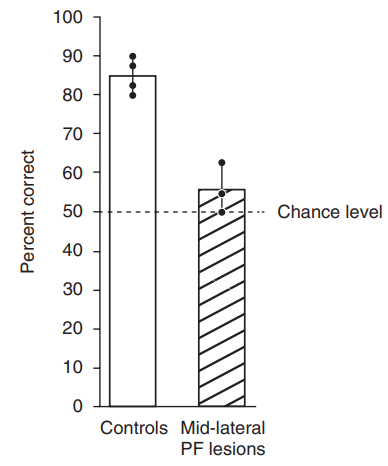
\includegraphics[width=0.3\linewidth]{image_pfc/Fig_6_4}
	\caption{来自有序对象任务的结果,也称为自有序任务。正常 (对照) 猴子 (白条) 和有病的猴子 (孵化条) 的正确率。填充的圆圈表示每个主题的表现,用垂直线表示范围。从Petrides M.重新绘制。猴子外侧额叶皮质中背部分病变后,对非空间自序和外部有序工作记忆任务的损伤。神经科学杂志15:359-75,©1995神经科学学会,经许可。}
	\label{fig:fig}
\end{figure}
\subsection{总结}
在涉及对象的任务中,每个试验使用不同的项目时,具有中外侧PF皮层病变的猴子表现正常; 但是,当实验者从试验到试验使用相同的刺激集时,病变的猴子的表现接近偶然水平。当然,在延迟响应和延迟交替任务中,实验者使用从试验到试验的同一组地点,而受损的猴子也具有接近偶然的水平。因此,未能解决审判间的干扰可能会导致延迟响应和延迟交替任务的损害。

然而,结果没有区分对干扰易感性的三种可能解释:
\par
1.猴子在判断事件的时间顺序时可能会出错。
\par
2.他们可能不知道指导任务执行的规则。
\par
3.他们可能无法通过对目标进行前瞻性编码来补偿干扰。

我们将在接下来的三个部分中依次讨论这些可能性。

\section{时间顺序}
第一种解释表明,具有中外侧PF病变的猴子在区分两种刺激事件中的哪一种方面存在障碍,例如最近出现的左提示与右提示。随着一系列试验的展开,它们按时间顺序发生,只有一个是最近的。可以通过要求猴子根据发生的顺序在两个项目之间进行选择来测试一下第一个解释。在每次试验中使用不同的物品消除了干扰影响。

Petrides (1991) 做了这个实验,要求猴子选择更早而不是更晚出现的物体。他以给定的顺序提出了四个对象,后来又同时提出了两个对象作为选择。他在每次审判中都使用了新颖的物品。受害的猴子可以在序列中的第一项与任何替代项之间正确选择,或者在最后一项与任何替代项之间正确选择。但是这些选择并没有告诉我们什么,因为选择第一个刺激总是会带来回报,就像避免系列中的最后一个刺激一样。

在关键测试一下中,猴子必须在系列中间发生的项目之间进行选择。在四项系列中,第二项和第三项占据了这个中间地带。Petrides发现,中外侧PF皮质的背侧部分 (区域46) 的损伤在基于顺序区分项目方面造成了损害,特别是对于第二和第三项目 (图6.5)。他在五项系列中获得了类似的结果。
\begin{figure}
	\centering
	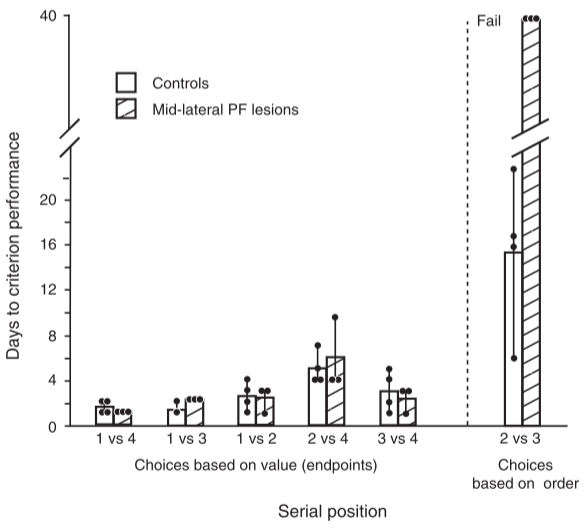
\includegraphics[width=0.5\linewidth]{image_pfc/Fig_6_5}
	\caption{串行时序任务的结果。在图6.4的格式中,除了纵坐标绘制了掌握问题的天数。根据它们在一系列项目中的排名,每对条将正常 (对照) 猴子 (白条) 和损伤猴子 (阴影条) 进行比较,以在两个项目之间进行选择 [1... 4]。垂直线虚线将涉及端点项 (项目1或4) 的选项与不包括端点的选项分开。对于后者,具有中外侧PF皮质病变的猴子在测试天数 (失败) 的限制内未掌握问题。重新绘制自Petrides M.背外侧额叶皮层内的功能专门化,用于序列顺序记忆。皇家学会学报-生物科学246:299-306,©皇家学会,1991,经许可。}
	\label{fig:fig}
\end{figure}
猴子可以学习这项任务,但只有困难。人类受试者发现使用一系列新颖的图片很容易学习任务。Milner等人 (1985) 报道,额叶切除术的患者在选择最近发生的图片方面表现不佳。他们不太可能失败,因为他们不知道规则,因为在每次试验中,实验者都要求他们选择最近的照片。

当然,这种损害可能是由这些大病变的任何部分引起的。因此,Amiez和Petrides (2007) 对人们进行了成像实验,因为他们判断两个刺激中的哪一个在序列中较早出现。激活发生在PF中外侧皮层。

中外侧PF皮层中单细胞编码顺序的发现支持了病变和激活研究。Ninokura等人 (2003) 依次呈现了三种彩色图案,猴子学会了按此顺序触摸它们。在中外侧PF皮层中,43\% 具有延迟周期活性的细胞编码了出现图片的序列。Funahashi等人 (1997) 发现了空间刺激的相似结果。他们的猴子必须按照它们出现的顺序选择两个目标,以及表现出延迟期活性的中外侧PF皮层细胞,62\% 编码的刺激顺序。

Warden和Miller (2007) 的一项研究提出了一种可能的顺序编码机制。他们记录在中外侧PF皮层,而猴子执行一项任务,他们必须判断最近发生的两张照片中的哪一张。第二张图片的活动超过了第一张图片的活动,该属性可以提供判断顺序的机制。
\subsection{总结}
由于无法判断事件的顺序,可能会导致延迟响应任务的损害。在一系列试验中,视觉事件指导着每个可能目标的选择,只有最后一个与当前试验相关。本节回顾了具有中外侧PF病变的猴子在区分事件顺序方面存在障碍的证据。同样,中外侧PF皮层中的细胞编码事件顺序。回想一下,Tsujimoto和Postle (2012) 表明,当猴子在延迟响应任务的动眼运动版本中犯了坦率的错误时,他们通常会选择先前试验中合适的目标 (第5章)。

\section{规则}
我们对损害的第二种解释表明,受损的猴子无法学习或应用任务规则。要执行延迟响应任务,猴子必须以某种形式应用以下规则: 最近的视觉事件的位置确定当前目标。

猴子可以学习许多这样的规则,我们知道,当猴子学习一个规则时,中外侧PF皮层中的细胞会像在PF皮层的其他部分一样编码这些规则。第7章针对腹侧PF皮层详细介绍了此问题。例如,PF皮层中的细胞对条件视觉运动规则和空间规则 (白色和Wise 1999) 具有不同的活性。单元格的编码匹配或不匹配规则(Wallis等人2001) 以及匹配规则是否涉及颜色或形状 (Mansouri等人2006)。此外,PF神经元前瞻性地编码这些规则,即在其实现之前 (Wallis等2001)。

Buckley等人 (2009) 的一项研究支持了中外侧PF皮层在执行任务规则中的作用。他们测试了已经学习了两个版本的匹配样本任务的猴子。在一个版本中,猴子根据形状进行匹配; 在另一个版本中,它们根据颜色进行匹配。在每次试验中,他们选择了三种刺激: 一种是按颜色匹配样本,另一种是按形状匹配样本,另一种是不匹配特征。一旦动物达到一条规则的标准,实验者就会通过仅包含奖励或非奖励的反馈来提示切换到另一条规则。

猴子在手术前学习了这些规则,并且具有中外侧和后外侧PF皮质病变的猴子可以重新学习并在它们之间切换。但是,如果在他们重新学习了其中一条规则之后,他们遇到了比通常更长的审判间隔,则他们的表现50\% 正确 (Buckley等人2009) (图6.6)。此性能水平与机会水平相对应,前提是人们忽略了不遵循任何规则的选择。这一发现向Buckley等人暗示,中外侧PF皮层在维持内存中的当前任务规则中起作用。
\begin{figure}
	\centering
	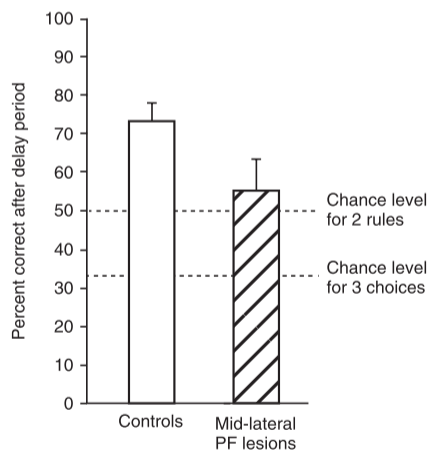
\includegraphics[width=0.5\linewidth]{image_pfc/Fig_6_6}
	\caption{猴子在规则任务上的表现类似于威斯康星卡片排序任务。猴子执行与样本匹配的任务,按颜色或形状进行匹配,在试验块中交替进行。延迟期后,正常 (对照) 猴子 (白条) 和中外侧PF皮层 (阴影条) 病变的猴子的正确性能百分比从6s增加到11s。虚线显示了整个任务 (正确33\%)和遵循两个规则之一的选择 (正确50\%) 的性能的机会水平。误差条: SEM。修改自Buckley MJ,Mansouri FA,Hoda H,Mahboubi M,Browning PGF,Kwok SC,Phillips A,Tanaka K。规则指导行为的可分离成分取决于不同的内侧和前额叶区域。科学325:52-8,©2009 AAAS,经许可转载。 }
	\label{fig:fig}
\end{figure}
其他证据表明,背侧PF皮层 (包括外侧区域9,中外侧和后外侧PF) 在学习规则中起作用。关于延迟交替任务的规则之一是,如果猴子犯了错误,则奖励将在下一次审判中位于同一侧。此规则之所以适用,是因为标准的延迟交替任务使用了纠正程序,这有助于动物掌握任务。这意味着猴子可以采取一种称为 “迷失” 的策略,以帮助他们解决问题。根据此规则,当一个目标的选择未能得到回报时,该目标应在下一次判断中被拒绝。

Passingham (1975) 分析了背侧PF皮质病变的猴子在延迟交替任务上的错误。在测试的三只动物中,一只进行了420试验来学习 “迷失” 策略,一只进行了900试验,一只在1000试验中没有学习。相比之下,两只正常的猴子花了240和60来学习相同的策略,而一只猴子不需要训练就可以应用该规则。因此,具有背侧PF病变的猴子在获得 “迷失转移” 策略方面存在严重障碍。

一旦猴子学会了纠正试验的 “失速策略”,他们就需要学习延迟交替任务的常规试验规则。此规则定义了任务: 每次试验的目标应该是在先前试验中没有奖励的地方。换句话说,他们必须学习 “双赢” 规则。与诸如 “双赢” 或 “亏损” 之类的规则相比,“双赢” 规则具有任意性质。强化使动物更有可能选择一个有回报的目标,而 “双赢” 规则支持这一原则。同样相反的是 “迷失转移”。然而,“双赢” 规则反对最近的加固历史。在Passingham (1975) 的研究中,具有背侧PF病变的猴子在1000试验中未能学习 “双赢” 规则。
\subsection{总结}
延迟响应和延迟交替任务的损害可能反映出未能应用适当的任务规则。延迟响应任务使用以下规则: 最近的视觉事件确定猴子应选择的目标: 其选择应与该事件的位置匹配。延迟交替任务使用的规则是,应该拒绝最近的目标选择,而选择替代方案。

这种可能性与第4章讨论的关于选择-结果关联的信用分配的想法有间接的关系。具有眼眶PF病变的猴子在单个事件的基础上在学习选择结果关联方面存在障碍。可能是,具有中外侧PF皮质病变的猴子有一个相关的问题: 也许他们无法实现使用单个事件 (最近提示的位置) 来生成当前目标的规则。

\section{前瞻性编码}
早些时候,我们提出了第三种解释损伤对延迟反应任务的影响。也许具有中外侧 PF 皮层损伤的猴子可以学习这一规则,但不能通过前瞻性地编码记忆中的目标来补偿记忆中的干扰。根据这种观点,对当前目标的短期记忆可以避免一审接一审的干扰。
\begin{figure}
	\centering
	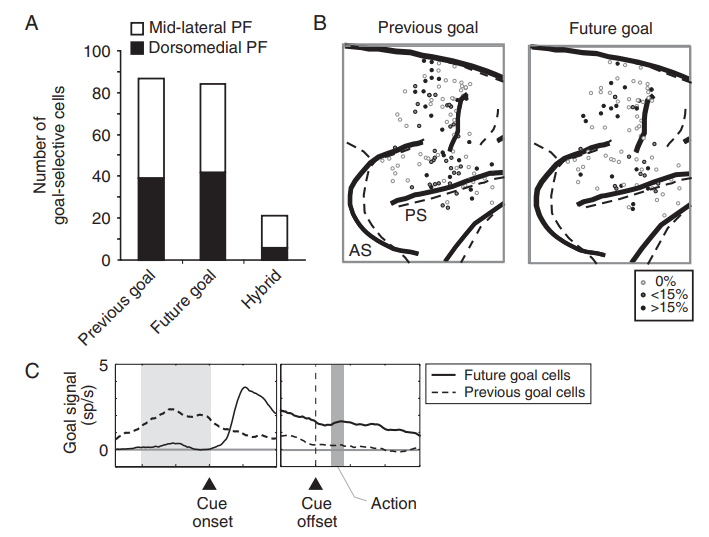
\includegraphics[width=0.5\linewidth]{image_pfc/Fig_6_7}
	\caption{独立的编码之前和现在的目标。(一)大多数PF神经元编码当前目标或者上一个,只有几个编码(混合)。这些数据表明,PF皮层细胞编码回顾性和前瞻性记忆。(B)的位置细胞编码以前或现在的目标。空圆圈显示网站没有这样的编码;光明与黑暗的灰色圆圈显示网站小于15\%或大于15\%的神经元显示这些属性,分别。虚线显示第二个猴子的沟,叠加在那些从第一(固体沟的行)。(C)目标信号之前和现在的目标人口水平。虚线显示平均为回顾性编码信号;黑色的线显示了潜在的意思是信号编码。改编自Genovesio Brasted PJ,明智的SP。表示未来和以前的空间目标的单独的前额叶皮层的神经种群。神经科学学会神经科学杂志》上26:7305-16,©2006年许可。}
	\label{fig:fig}
\end{figure}
在一项研究中已经提到,Genovesio (2006 a)记录的神经元活动的两个部分背PF皮层(面积46和9)(图6.7 B)。在每个试验中,这只猴子已经选择在三个空间目标:左,右,注视点。也在这一实验中,这只猴子已经使用回顾性记忆最近的目标选择的当前目标的选择(前瞻记忆)(图6.7摄氏度)。

Genovesio 等人在背侧 PF 皮层发现了两个独立的细胞群。一个编码目标在前一个试验中的位置,另一个编码目标在当前试验中的位置(图6.7 A)。只有少数细胞编码位置更一般(杂交细胞)。病变的影响可能因此使动物无法区分过去和现在的目标,因为在前瞻性编码失败。如果无法单独区分以前目标和现在目标的位置,就会造成延迟响应任务的不足。动作中外侧 PF 背内侧 PF B 先前目标未来目标 PS 目标信号(sp/s)目标选择细胞先前目标未来目标杂交。
\begin{figure}
	\centering
	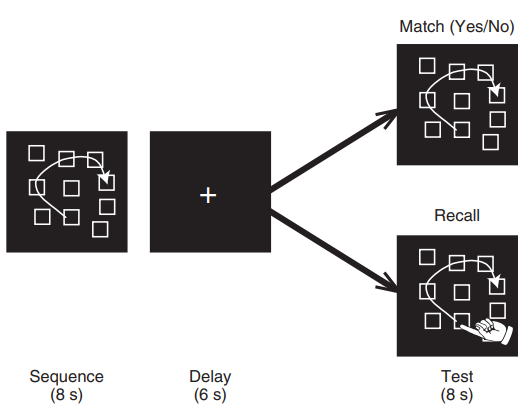
\includegraphics[width=0.5\linewidth]{image_pfc/Fig_6_8}
	\caption{在成像实验中使用的匹配和回忆任务。在展示了一系列的位置(左图,弯曲的箭头)和一个延迟时间(中间)之后,受试者需要执行两个任务中的一项(右图)。在顶部的分叉中,受试者看到一系列的空间线索,并必须报告它是否与最初呈现的线索相匹配,称为匹配条件。在底部的分叉中,受试者必须复制最初观察到的序列,称为回忆条件。只有在回忆条件下,受试者才会在延迟期间计划出一系列目标的动作。背外侧前额叶皮层在即将到来的行动准备中的作用:功能磁共振成像研究。大脑皮层11:260-6,©2001;经牛津大学出版社许可。}
	\label{fig:fig}
\end{figure}
对人类研究对象的研究也为中外侧PF皮质的前瞻性编码提供了证据。Pochon等人(2001)研究了受试者执行两项任务来测试记忆序列时的激活。视觉刺激出现在多达5个位置的序列中,在延迟6秒后,实验者通过两种方式之一来评估记忆(图6.8)。首先,他们在延迟后呈现另一个序列,被试必须按下一个按钮来报告它是否与原始序列相匹配。第二,在延迟期之后,受试者必须按照他们出现的顺序指向每个位置。他们称为第一个条件匹配和第二个条件回忆。

在匹配条件下,受试者在延迟期间不知道是否会按下按钮。因此,这种情况要求他们记住感觉线索(回顾性记忆) ,但排除了未来行动的计划(前瞻性编码)。相比之下,在回忆条件下,受试者可以在延迟期间准备他们的行动(前瞻性编码)。

Pochon等人发现,在匹配条件下,尽管需要记住一系列线索位置,但在中外侧PF皮层中没有显著的延迟期激活。相反,在回忆条件下,他们发现该区域的延迟期激活非常显著(图6.9)。匹配和回忆条件都需要回顾性空间记忆。条件的不同之处在于,回忆条件要求计划未来的一系列目标或行动:前瞻性编码。
\begin{figure}
	\centering
	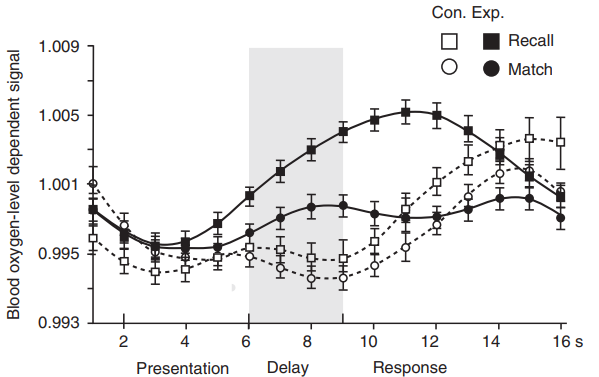
\includegraphics[width=0.6\linewidth]{image_pfc/Fig_6_9}
	\caption{在图6.8中所示的任务中的成像激活。填充方块:召回条件;未填充方块:召回条件控制;填充圆:匹配条件,未填充圆:匹配条件控制。误差条: S.E.M.最大的延迟期激活,在11秒达到峰值,当受试者计划一系列空间目标(回忆任务)。背外侧前额叶皮层在即将到来的行动准备中的作用:功能磁共振成像研究。大脑皮层2001年;11:260-6,经牛津大学出版社许可。}
	\label{fig:fig}
\end{figure}
Pochon等人还发现,在尾侧PF皮层和后顶叶皮层中存在延迟期激活。然而,在这些区域,激活发生在匹配任务和回忆任务,任务之间没有差异。因此,中外侧PF皮层与尾侧PF和后顶叶皮层在回顾性编码(匹配过程中)缺乏明显的显著激活,这表明PF激活的特殊之处涉及前瞻性编码。

同样的研究人员追踪他们的实验设计任务有两个延迟时间(Volle et al . 2005年)。受试者再次看到一系列位置,他们必须记住。只有第二延迟周期允许未来的目标的潜在编码。显著的延迟周期mid-lateral PF皮层的激活发生在第二次延迟周期而不是第一个。在一个控制任务中,一个新的序列连续第二次延迟周期期间出现在屏幕上,和受试者准备执行序列代替原来的。如果延迟周期激活反映了计划为未来的目标序列,而不是前一顺序的记忆线索,然后每个人都应该看到相同的激活控制任务的主要任务,而这正是Volle等人发现的。

大家可以反对,明显缺乏延迟期激活在第一延迟期是由于不敏感的 BOLD 信号。而事实上,戈德曼-拉基奇和梁(2002)提出了这个反对当罗et al .(2000)报道缺乏delayperiod激活空间记忆任务。在任务被罗等人受试者可以记住刺激延迟期间,但他们不能前瞻性编码的目标。

有可能测试是否缺乏延迟周期激活是否是由于方法的不敏感性。Sridal和Curtis(2008)使用特殊的线圈来提高敏感性,他们可以在空间匹配任务中检测到背侧PF皮层(额上沟)的吻侧的延迟期激活。这一发现与猴子的细胞记录的结果一致。如前所述,Genovesio等人(2006a)在该区域发现了一个编码回顾性记忆的细胞亚群。因此,不能用成像结果来证明这种活动的缺失。相反,他们认为在中外侧PF皮层(第46区)的前瞻性激活优于回顾性激活,这可能是基于更大程度的突触活动(第1章)。

鉴于在中外侧PF皮质中回顾性编码位置的细胞,我们的观点的批评者仍然可以声称这种活动支持回顾性工作记忆。(1998)在Pochon等人后来使用的任务上测试了背侧额叶皮层损伤的患者。他们发现患者在匹配条件下没有损伤,不涉及目标前瞻性编码的情况。原因可能是后顶叶皮层的细胞可以支持位置记忆。然而,正如成像结果所预期的那样,相同的患者在回忆条件下有障碍,涉及对目标进行前瞻性编码的条件(Ferreira等人,1998)。等人(2006)也报道了背额叶损伤的患者在回忆来自一系列位置的序列时具有损伤。因此,本节中的所有研究都指出了前瞻性编码在中外侧PF皮质功能中的重要性。

\subsection{预期的编码和干扰}
我们建议未来编码补偿干扰在内存中。累加器网络的概念,如第3章介绍,说明了这是如何工作的。第五章用这个概念来解释自顶向下竞争之间的偏见表示关注。根据这种观点,PF的影响皮质类似一个“规模拇指”为一种感官的代表提供一个优势与另一个集成“证据”对一个阈值。延迟反应任务,最近有关视觉事件作为至关重要的“证据”代表目标适合一个累加器网络事件。如果最近的线索或食物出现,例如,这个事件提供了足够的“证据”的生成一个目标。自顶向下的注意第5章的区别和自顶向下的注意延迟反应任务是,前者涉及感官处理,后者涉及目标的一代。成功的表现,最近的事件的记忆,右边的提示在这个例子中,必须在竞赛中获胜的内存更少的最近的事件,如早期的线索。

在一项针对人类研究对象的研究中,Sakai等人(2002a)通过故意在任务中引入干扰物来测试这一建议。受试者看到了五个空间位置的序列,在一半的试验中,在一个可变的延迟期之后,又出现了5个干扰物的位置(图6.10A)。在呈现干扰物后,实验者测试被试的记忆:首先是干扰物项目的顺序,然后是原始项目的顺序。
\begin{figure}
	\centering
	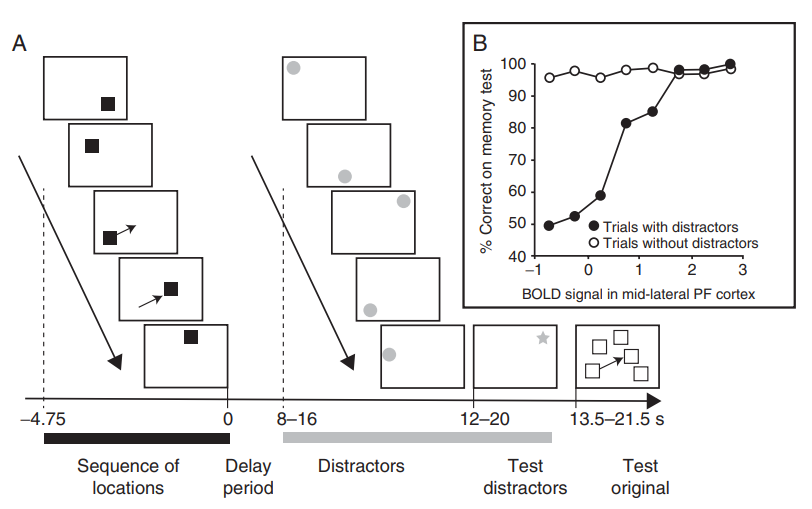
\includegraphics[width=0.6\linewidth]{image_pfc/Fig_6_10}
	\caption{空间记忆任务在成像实验中的应用。填充的黑色方块表示空间线索的原始序列; 填充的灰色圆圈表示一系列干扰物。有些试验缺乏干扰因素。灰色的星星代表一个探测器的干扰项目。受试者必须说出这个位置是否是干扰器系列中的一个。在这个例子中,它是(从顶部开始的第三个)。右下方面板中的箭头显示了从一个位置到另一个位置的可能转换。受试者必须说明这种转变是否发生在原始序列中。在示例中,它做到了,正如左栏第三和第四面板中的箭头所指出的那样(受试者没有看到)。(B)性能准确性作为中外侧 PF 皮层激活(BOLD 信号)在延迟期间的功能。填充圆圈: 有干扰物的试验; 未填充圆圈: 没有干扰物的试验。受试者事先不知道是否会出现干扰物。改良自 Sakai K。主动维持前额区46能产生抗干扰记忆。自然神经科学杂志5:479-84,2002,自然出版集团。}
	\label{fig:fig}
\end{figure}
尽管匹配过程测试内存,使用长延迟迫使科目演练项目。Tremblay et al。(2006)表明,当允许这样做的时候,主题往往通过他们的眼睛从一个位置移动到另一个地方。当然,人们可以记住位置没有采用这个策略,但是排练地点以这种方式帮助他们保留信息,如图所示,如果对象移动他们的眼睛在延迟无关紧要的位置,他们也不记得项目(Guerard et al . 2009年)。

Sakai et al。(2002)使用长延迟和发现显著延迟周期激活mid-lateral PF皮层,即使使用了一个匹配的过程。这支持他们所担负的序列。梁et al。(2002)也使用一个匹配的过程长延迟(18或24秒),和他们也发现延迟时间越长,分心的可能性就越大,因此熟练的动机就越大。

在Sakai等人(2002a)的研究中,延迟在8-16秒之间变化,直到5秒后才进行了对该位置的记忆测试。此外,受试者不知道在任何给定的试验中是否会出现干扰物。图6.10显示,在使用干扰物的试验中,延迟期激活的程度与受试者反应的准确性密切相关(图6.10B)。这些结果表明,延迟期激活可以保护记忆不受干扰。

这项研究刚刚描述了所使用的位置作为刺激物。Sakai和帕辛汉姆(2004)随后使用字母作为刺激物,以操纵干扰的程度。他们通过使用与记忆项目相同或不同的干扰物来做到这一点。和之前的研究一样,实验者展示了五个要记住的字母的序列,然后是一个延迟。然后,他们以另外五个字母或五个数字作为干扰物,然后测试原始字母。显然,带有干扰物的字母比数字产生了更多的干扰。

在早期的研究中,Sakai等人(2002b)发现中侧 PF 皮层的延迟期激活。在记忆测试期间,在检索原始字母序列时也发生了激活。重要的是,高干扰条件(字母干扰器)比低干扰条件(数字干扰器)产生显著更大的激活。这一发现支持这样的观点,即前瞻性激活中外侧 PF 皮层可以帮助保护记忆免受干扰。
\subsection{总结}
我们对受干扰敏感性的第三个可能的解释援引了勘探的概念。本节提出的证据表明,预期编码,以细胞活动和区域激活的形式,发生在中外侧PF皮层。我们不否认这一区域的一部分细胞反映了延迟期间的回顾性编码,但至少在成像数据中,前瞻性编码似乎占主导地位。

我们提出,中外侧PF皮层的前瞻性编码可以补偿记忆中的干扰。随着延迟期激活的增加,面对干扰的记忆变得更加准确。而随着干扰的增加这些发现支持了这样一种观点,即中外侧PF皮质受损的猴子在回忆时会出现激活增加。外侧PF皮质屈服于干扰,因为它们不能前瞻性地编码当前目标。

综合最后三个主要部分,我们得出结论: 中外侧 PF 皮层损伤导致延迟反应和延迟交替任务的损害,其原因有三个相关原因中的一个或多个。首先,他们可能已经失去了区分最近相关事件和早期事件的能力。其次,他们可能无法学习或实现任务规则,这些规则要求使用最近的事件来选择当前目标。第三,他们可能无法通过对当前目标进行前瞻性编码来弥补近期试验的干扰。我们将这三种可能性分别称为顺序编码、规则编码和预期编码帐户。

\section{目标产生}
我们不知道顺序编码、规则编码或前瞻性编码这三种可能性中的哪一种是导致中外侧前部皮层(46区)损伤后延迟反应损伤的原因,也许它们都是导致延迟反应损伤的原因。不管怎样,所有这些任务的一个关键因素是猴子必须在不同的试验中改变他们的目标选择,人体实验也有相同的要求。

我们早就知道,如果受试者产生一系列动作,尽可能随机地改变它们,中外侧前部皮层就会被激活。在Deiber等人的研究中(1991),受试者在四个方向中的一个移动操纵杆,在Frith等人的研究中(1991)他们移动了两个手指中的一个。在这两项研究中,受试者决定在每种情况下做什么动作。这导致人们认为这些任务涉及“自由选择”(Playford et al . 1992)或“意志行动”(Frith et al . 1991)。

自这些研究以来,出现了更多的研究,并且都发现了相同的结果(Spence \& Frith 1999;弗里思2000)。此外,正如Rowe等人(2005)所表明的那样,当受试者产生手指运动时,不仅中外侧PF皮层被激活,而且当箭头方向指示运动时,这种激活不会发生。

考虑到受试者在不同的试验中动作不同,他们需要注意最后几个动作。因此,在延迟反应和延迟交替任务中,每次试验的选择取决于先前的选择。

Barraclough等人(2004)的一项神经生理学研究同样要求猴子在左目标和右目标之间做出一系列选择。一个计算机程序决定一个选择是否会得到奖励,它会随着时间的推移而改变,以鼓励猴子切换目标,很像第四章回顾的对象逆转任务。作者记录了中外侧前部皮层,发现了相当大比例的细胞在之前的试验中编码了选择,以及其他信息。例如,只有当前一个目标在左边时,一个单元格才可能编码一个在右边的目标。许多细胞也会对之前的选择是否产生了奖励进行编码。这些细胞整合了关于先前选择及其结果的信息。Barraclough等人得出结论,他们更新了一个决定当前选择的价值函数,就像第4章讨论的眶前皮层中的细胞一样。

Tsujimoto和Sawaguchi (2004a, 2005)发现有证据表明,中外侧PF的细胞编码目标和结果的组合,Tsujimoto等人(2011a)也得到了类似的结果。后一项研究的任务包括一个视觉线索,提供一个从之前的空间目标转移或停留的指令。如图6.11所示,最上面的单元格编码了之前的目标,下一个单元格编码了未来的目标,下一个单元格编码了策略和目标的结合,最下面的单元格在得到提示后立即编码了策略,然后又改变编码了当前的目标。

因此,细胞记录结果与成像结果一样,支持了中外侧前部皮层在产生目标中起作用的建议。这些结果也指向一系列事件的重要性,包括在连续试验中出现的目标和线索。通常,一次试验的目标取决于之前试验的结果。
\begin{figure}
	\centering
	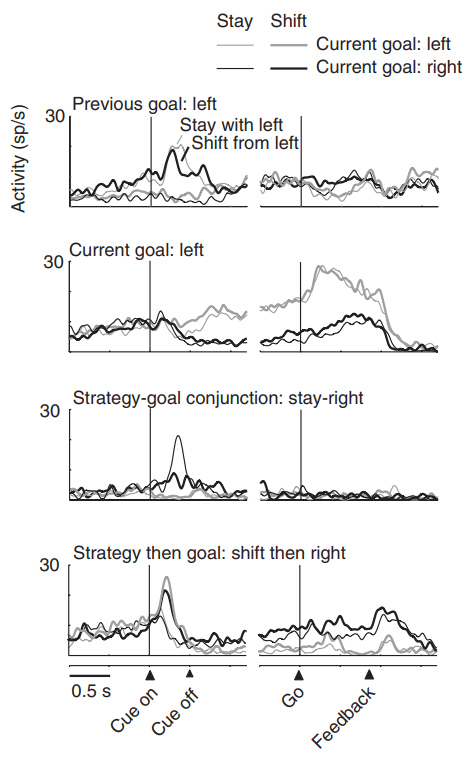
\includegraphics[width=0.3\linewidth]{image_pfc/Fig_6_11}
	\caption{提示策略任务中中外侧前额皮质活动模式。四个单元格中的每一个都显示不同的编码属性。细线显示的是停留提示下的平均细胞活动;粗线表示移位提示的活动。灰线表示导致选择当前目标的试验活动;黑线在右边表示当前目标的活动。线索类型和先前目标的组合决定了每次试验的当前目标。例如,对于顶部的单元格,细灰线显示了带有停留提示的试验活动,左边是先前的目标,因此左边是当前的目标。顶部的单元格也更喜欢带有移动提示的试验,将之前的目标移到左边,因此将当前目标移到右边(移动)。细胞活动的共同特征是,它会对左边的前一个目标进行编码。下一个单元格倾向于左侧的当前目标(灰线);下一个更倾向于将停留策略和当前目标结合在一起(细黑线);底部的单元格在提示期间编码移动策略(粗线),但在试验后期编码向右当前目标的选择(黑线)。来自Tsujimoto S, genvesio A, Wise SP的数据。背外侧和眶侧前额皮质策略信号的比较。神经科学学报31:4583-92,©2011,美国神经科学学会。}
	\label{fig:fig}
\end{figure}
如果每次试验的顺序不同是至关重要的,那么一个简单的预测就出现了:在这些任务的第一次试验中,活动和激活应该是缺失的。首先,第一次试验与前一次试验没有任何不同。第二,第一次试验的选择不依赖于前一次试验中的任何事件。在第一次审判中,没有最近发生的事件提供做出选择的背景。

因此,Rowe等人(2010)在一系列手指运动的第一次试验中检查了激活。正如预期的那样,在这项任务中,激活发生在中外侧前部皮层,这在许多试验中是平均的。但至关重要的是,在第一次试验中,该区域没有出现明显的激活。这一结果并不反映该方法缺乏统计能力或灵敏度;当作者在这个系列的中间选择一个单一的试验时,他们可以检测到中外侧前部皮层的显著激活。

如果这种激活在不同系列的产生中起关键作用,那么PF皮质大损伤的患者在“自由选择”任务中应该受损。Johns(1996)收集了20个这样的病人,让他们用一个可以向四个方向移动的操纵杆做一系列的动作。与对照组相比,患者产生了更多的刻板印象和更少的随机动作序列。

Johns等人的研究涉及较大的病变,但成像和重复经颅磁刺激(rTMS)可以更准确地定位关键区域。Jahanshahi等人(2000)观察到,当受试者随机生成一系列数字时,中外侧前部皮层被激活,随机序列越多,激活程度越高。在随后的一项研究中(Jahanshahi \& Dirnberger 1999),同样的研究人员将rTMS应用于该区域以破坏其活动,这种损伤导致该系列变得更加刻板化。因此,中外侧前部皮层似乎在不同试验中做出不同的选择时发挥了必要的作用。

\subsection{总结}
本节与前三节一样,回顾了中外侧前部皮层根据事件顺序产生目标并对目标进行前瞻性编码的证据。首先,当人们产生一系列目标时,中外侧前部皮层会被激活。第二,激活反应了产生一系列不同目标的需要。第三,它似乎在一个系列的第一次审判中缺席。

\section{计划一个序列}
在前一节描述的任务中,受试者在试验中产生一系列目标。然而,我们并不总是知道他们是否只是在每次试验中产生下一个目标,还是他们事先计划了一系列目标。

为了找到答案,Averbeck等人(2006)教猴子三次眼球运动的序列,它们通过反复试验来学习。猴子可以在几次试验中学会这么短的序列。作者记录了前额叶皮层的后外侧,前额叶视野(FEF)的吻侧,并发现了编码特定序列的神经元的猴子在做出动作之前就计划好了。通过一种简单的解码算法,他们可以预测猴子什么时候会犯错误,以及错误是什么。这些结果表明猴子提前计划了一系列的动作。

在一项相关研究中,Shima et al(2007)教授猴子一系列动作。在他们的实验中,猴子做的是伸手的动作,而不是眼球的动作,他们操纵一个可以转动、推或拉的把手。每个序列由四个动作组成。每天,猴子通过视觉线索学习一个序列,然后根据记忆重复它。当猴子准备产生各种序列时,Shima等人从后侧前额皮质进行了记录。通常,在执行序列之前会有一段延迟期。

在与任务相关的细胞中,超过40\%的细胞表现出延迟期活动。Shima等人(2007)总共训练了11个序列,它们可以比较具有相似模式的序列。在这个意义上,模式指的是序列中的转换。例如,一个模式由双重复组成,AABB,其中a和B代表序列中的不同元素。另一种模式由交替组成:ABAB。这两个序列都由相同的元素组成,比例相同,但它们在过渡次数上有所不同。当然,A和B在不同的序列中是不同的,除此之外还有第三个刺激。

在不同序列表现出不同活性的细胞中,超过一半的细胞在相似模式的序列中表现出相似的活性。例如,作者举例说明了一个神经元,它编码了双重重复序列“转,转,推,推”和“拉,拉,转,转”,但没有编码重复序列:“转,转,转,转”或“拉,拉,拉,拉”。该细胞更倾向于AABB模式而不是AAAA模式。Shima等人将这一结果解释为序列类别的编码,如双重复(AABB)、交替(ABAB)或重复(AAAA)。在具有延迟期活动的细胞中,大约一半的细胞表现出特定类别的活动(图6.12)。Shima等人发现这些细胞在主沟背侧比在主沟腹侧多。

在目前所考虑的序列中,实验者指定了序列中元素的顺序。但是我们可以修改任务,让猴子从一个目标开始,并且必须找出实现这个目标所需的一系列元素。例如,Mushiake等人(2001)向猴子展示了一个视觉迷宫(图6.13),任务要求它们使用手柄将光标移动到迷宫的最终目标。

一旦猴子学会了一系列成功的动作,实验人员就会引入一个新的视觉障碍,这样猴子就必须规划一条新的路线。Mushiake等人记录了中外侧前部皮层的活动,包括主沟的背侧和腹侧,他们的分析集中在运动前的延迟期。在延迟期间,细胞对当前目标进行编码。如果实现最终目标需要三个从属目标的序列,则不同的细胞亚群为每个目标编码(Mushiake et al . 2006)。通过操纵手柄和光标运动之间的空间变换,Mushiake等人可以测试一个特定的细胞是编码一个从属目标还是一个特定的肢体运动。例如,手柄向左移动可以根据当前生效的空间变换,使光标向左或向右移动。而且,正如预期的那样,大多数细胞都为目标而不是运动编码。
\begin{figure}
	\centering
	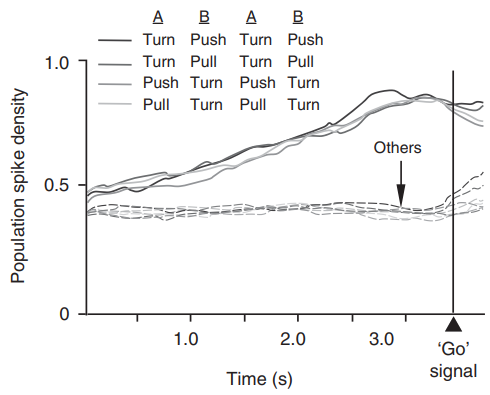
\includegraphics[width=0.4\linewidth]{image_pfc/Fig_6_12}
	\caption{背侧前部皮层细胞序列编码。实线表示这个神经元的首选序列,所有这些序列都遵循一个交替的模式:ABAB,不同的运动组成了这个序列。虚线表示不遵循这种交替模式的序列。经麦克米伦出版有限公司许可修改。李建军,张建军,张建军,等。脑皮层行为序列的分类。Nature 445:315-18,©2006,自然出版集团。}
	\label{fig:fig}
\end{figure}
\begin{figure}
	\centering
	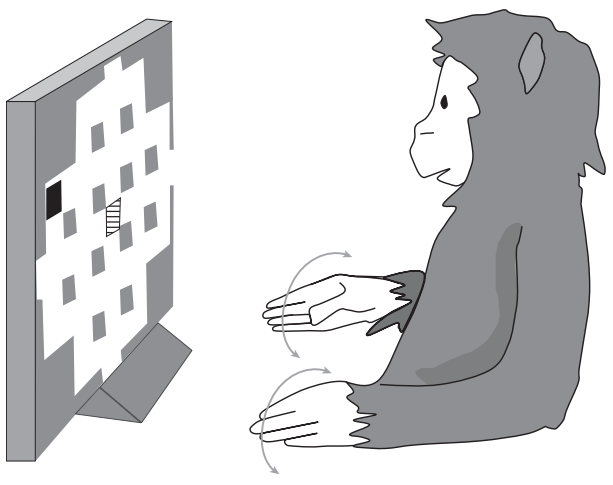
\includegraphics[width=0.4\linewidth]{image_pfc/Fig_6_13}
	\caption{视觉迷宫任务。猴子需要通过手部动作将光标从当前位置(灰色方块)移动到最终目标(黑色方块)。实验者可以改变手的运动来产生给定的光标运动。重新绘制自Mushiake H, Saito N, Sakamoto K, Sato Y和Tanji J.认知脑研究11:165-9,©2001,经爱思唯尔许可。}
	\label{fig:fig}
\end{figure}

为了解决迷宫任务所带来的问题,猴子必须计算从属目标和最终目标。中外侧前部皮层的细胞负责其中一种、另一种或两者的编码(Saito et al 2005)。这使得Sakamoto等人(2008)能够分离成对的细胞,其中一个编码从属目标,另一个编码最终目标。当一个神经元编码从属目标和另一个神经元编码最终目标之间发生转换时,放电的同步性达到峰值。同样,在要求使用先前目标选择当前目标的任务中,Tsujimoto等人(2008)发现编码当前目标的细胞与编码先前目标的细胞之间存在活动相关性。当猴子从之前的目标转移到之前的目标时,这些相关性会增强。

如果中外侧前部皮层在计划一系列目标中起着必要的作用,那么该区域受损的猴子应该在这些任务中表现出损伤。Passingham(1985)在Collin等人(1982)设计的空间搜索任务上测试了猴子。猴子坐在25扇门前,每扇门后面都放着一颗花生。猴子只需要伸手去打开一扇又一扇的门,取出花生。我们称之为25扇门搜索任务。

因为门是不透明的,所以这项任务要求猴子去够它看不见的目标。每扇门打开一次,而且只打开一次,因为实验者只有在经过很长一段时间后才会更换花生。正常的猴子很快就学会了这项任务。相比之下,前额皮质中外侧和后外侧受损的猴子更经常回到它们已经打开的门。他们的搜索模式显示出严重的混乱。

但这种混乱并不一定反映出计划的缺陷。这可能是由于没有记住他们已经打开了哪些门。Owen等人在两项损伤效应研究中排除了这一解释。他们用电脑版的空间搜索任务测试病人。额叶切除术患者受损;和猴子一样,他们倾向于回到已经试过的盒子。但是Owen等人也测量了他们搜索模式的一致性。他们推断,有规律地、有序地触摸这些盒子可以减少记忆负荷。前额叶受损的患者在选择开始搜索的盒子中表现出较少的规律性。由于这是第一个选择,这种不规则性不能归因于忘记了一系列的前一个选择,因此可以排除对结果的记忆解释。

定期搜索的一个好处是它减少了对工作记忆的需要。Taffe和Taffe(2011)为猕猴执行空间搜索任务开发了一个“策略得分”。猴子掌握了最小化动作之间距离的策略,如果没有使用这一策略,它们就会犯错。实验还没有完成,但根据25门搜索任务的结果,我们预计有中外侧前部皮层损伤的猴子的策略得分会很低。

我们在第2章和第5章中谈到了这种伸展运动的一个关键特征。我们解释说,在中央凹进化之后,灵长类动物发展了一种新的伸手方式,一种在注视中心坐标系中计算当前伸手目标和手的当前位置的方法(见图5.3)。我们提出,在类人猿进化出一种以注视为中心的坐标到达目标的机制后,这个系统成为以有序顺序到达目标的必要条件,特别是对于看不见的目标。为了达到可见的目标,运动前和顶叶机制就足够了,所以前部皮层的损伤不会影响这种行为。当我们稍后考虑为什么中外侧前部皮层在类人猿而不是其他哺乳动物的延迟反应任务中起必要作用时,这些观点变得重要起来(第10章)。

\subsection{总结}
前面的章节表明:(1)中外侧前部皮层根据事件的顺序、时间和位置提供的上下文产生目标,(2)它可以通过顺序编码、规则编码或预期编码来实现目标。本节将这个想法扩展到一系列目标。除了具体的目标,比如地点,中外侧前部皮层的活动反映了一个序列的抽象结构。因此,中外侧前部皮层既代表具体的目标,也代表抽象的目标,它既代表单个目标,因为它们在不同的试验中有所不同,也代表一系列目标,因为它们在结构化的序列中发展。中外侧前部皮层受损的人和猴子在组织序列方面表现出效率低下,这不能归因于记忆损伤。

随后,在第8章中,我们提出前额皮质可以编码抽象表征,因为它位于目标层次的顶端。在该层次结构的连续阶段,高阶细胞可以将来自低阶细胞的信息组合在一起。通过这种方式,前额叶皮层可以对目标的抽象表征进行编码。下一节认为,前额叶皮层也编码当前情境的表征。

\section{连词和当前语境}
在前面的章节中,我们已经讨论了当前上下文可以通过一系列事件的顺序和它们的空间位置来指定。但其他信息有助于当前的环境,背侧前部皮层也编码这些方面的视觉事件。

\subsection{时间间隔}
时间间隔的持续时间,就像事件在时间上的顺序一样,在建立行为环境中起着重要作用。后顶叶区LIP的细胞编码时间间隔的长度(Leon \& Shadlen 2003),该区域投射到背侧前额皮质。

因此,人们会期望在前皮层中发现反映时间间隔的活动。在最近的一项研究中,Yumoto et al(2011)从外侧区9的皮层记录。一盏灯在指定的时间内出现,猴子被训练在相同的时间间隔过后按下按钮来报告这个时间间隔。他们发现了两组神经元。在指定的时间过去后,一群细胞变得活跃。Genovesio等人(2006b)在猴子没有进食时发现了类似的结果报告时间间隔。Yumoto等人还发现,当猴子在没有外部提示的情况下复制时间间隔时,细胞变得活跃。

因此,我们可以预期,在繁殖的间隔时间内,有外侧9区损伤的猴子会受到损害。Passingham(1978)训练猴子报告它们按了一个键1次还是5次,Manning(1978)训练猴子报告它们按了杠杆32次还是64次。背侧前部皮层的损伤导致了这两项任务的损伤。这些缺陷可能反映了计数方面的困难,但似乎更有可能是计时方面的缺陷。

在Passingham(1978)的研究中,只有PF皮层中外侧和后外侧受损的猴子表现正常。这一发现表明,背凸皮质(侧区9)的切除导致了损伤。而且,Yumoto等人(2011)发现,侧区失活9会导致猴子在报告时间间隔时出现错误。

Yumoto等人在研究中报告的细胞活动仅反映了时间间隔。但我们也可以找到一些活动,它们反映了物体的身份和它们被呈现的时间之间的联系。Genovesio等人(2009)训练猴子区分相对持续时间,并从中外侧前部皮层的细胞中进行记录。一个蓝色的圆圈和一个红色的正方形出现在猴子的注视点,它们持续的时间不同。延迟一段时间后,两个刺激同时出现,一个在左边,一个在右边。为了获得奖励,猴子需要选择持续时间较长的那个。Genovesio等人发现,前部皮层背侧的细胞编码刺激特征和相对持续时间之间的连接。例如,许多细胞认为蓝色刺激持续的时间更长。

\subsection{距离}
我们提到后顶叶皮层的细胞编码时间间隔(Leon \& Shadlen 2003)。那里的一些细胞编码条的长度(Tudusciuc \& Nieder 2007)。因此,Genovesio等人(2011)记录了猴子在执行距离识别任务时中外侧前额皮质的活动。他们使用了和刚才提到的持续时间辨别任务相同的刺激物:一个蓝色的圆圈和一个红色的正方形。一种刺激出现在参考点上方的一段距离,另一种刺激出现在参考点下方的不同距离。猴子需要报告哪个刺激出现得离参照点更远。一些细胞编码绝对距离,但更多的细胞编码相对距离。而且,在持续时间辨别任务中,许多细胞编码的刺激特征与相对距离的连接。

如果背侧前部皮层在辨别距离方面起着关键作用,那么该区域受损的猴子在必须报告距离的任务中应该受到损害。Mishkin等人(1977)教猴子将杠杆移动两个不同的距离,然后通过在两个刺激中选择来报告距离。背侧前额皮质受损的猴子在这项任务中表现不佳。这个结果可能反映了对移动距离的错误判断,但也可能是由于判断移动持续时间的缺陷,或者两者兼而有之。

\subsection{连接}
我们已经说过,前部皮层背侧的细胞代表持续时间和距离,在前一节中,我们提到了一项研究,据报道,许多前部皮层细胞编码顺序(Ninokura等人2003;Genovesio et al . 2009)。考虑到背侧前部皮层接收来自后顶叶皮层的投影,并且那里的细胞编码相同的特征,这些结果不应该令人惊讶(Tudusciuc \& Nieder 2007;Bueti \& Walsh 2009)。

然而,前部皮层的细胞与后顶叶皮层的细胞在一个重要的方面有所不同。正如刚才提到的,前部皮层背侧的许多细胞编码特征连接。例如,后顶叶皮层的细胞编码持续时间,但中外侧前部皮层的细胞还编码刺激颜色和持续时间的结合。在Genovesio et al(2009)的研究中,猴子需要报告颜色和持续时间的关联,但它们不需要报告刺激顺序,比如第一个还是第二个刺激持续的时间更长。然而,中外侧前部皮层的许多神经元编码了相对持续时间和刺激顺序的关联。

同样,在同一作者(Genovesio et al, 2011)的后续研究中,猴子必须报告刺激颜色和相对距离的关联,但不需要报告顺序信息。然而,许多细胞同时编码这两种连接。较少数量的细胞编码刺激是高于还是低于参考点更远。这些发现表明,时间顺序在中外侧前部皮层的细胞活动中起着特别重要的作用。

图6.14显示了两个任务中基于顺序的连接词相对于目标的信号编码情况。时序表明基于顺序的连词在目标的生成中起中介作用。之后,许多细胞编码到达运动:达到目标的动作。

顺序-持续时间、顺序-距离和位置-距离连词并不是在中外侧前额皮质中观察到的唯一类型的整合。表6.1列出了在其他任务中发生在其神经元中的一些连接表征。例如,Hoshi和Tanji(2004)在一个序列中向猴子展示了两个线索,一个告诉他们到达左边或右边的目标,另一个告诉他们使用左臂或右臂。在中外侧前部皮层腹侧记录的细胞活动倾向于反映提示的空间方面,而在背侧记录的细胞倾向于反映手臂-目标连接。

因此,背侧前部皮层似乎是导致目标产生的多种信号的集合点。它发挥这种功能是因为它的连接:来自后顶叶皮层的输入传递空间、时间和顺序上下文,来自眶前部皮层的输入提供结果信息,前部皮层的内在连接提供其他类型的信号。
\begin{figure}
	\centering
	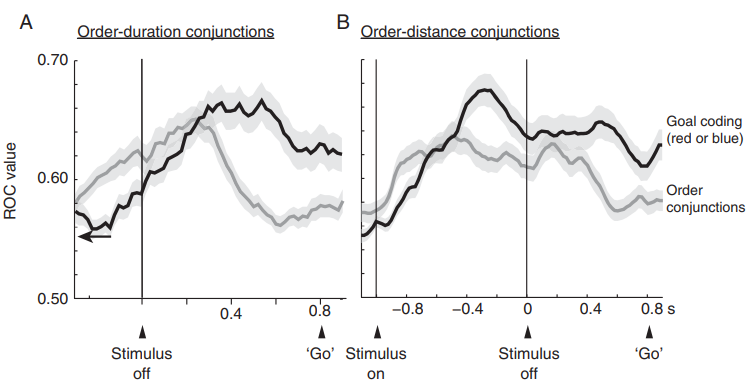
\includegraphics[width=0.5\linewidth]{image_pfc/Fig_6_14}
	\caption{前额皮质背侧编码连词的活动。(A)编码顺序和相对持续时间结合的细胞的种群活动(灰线)。这些细胞编码了在给定的试验中,两种刺激中的第一种还是第二种持续时间更长。材质:SEM。纵坐标表示接收者工作特征(ROC)在单个细胞上的平均值,它表示每个细胞编码给定顺序-持续时间连接的平均能力。箭头表示机会水平的ROC值。(B)相同皮层区域的顺序距离连接(灰线)。如图(A)所示。两幅图中的黑线显示了编码目标的活动,红色或蓝色刺激。(A)源自genvesio A, Tsujimoto S, Wise SP。}
	\label{fig:fig}
\end{figure}

\begin{table}[htbp]
	\newcommand{\tabincell}[2]{\begin{tabular}{@{}#1@{}}#2\end{tabular}} %换行指令
	\centering
	\caption{前额皮质背侧的连词编码}
	\renewcommand\arraystretch{1.5}	%设置表格内行间距
	\begin{tabular}{llll}
		\toprule 
		连接   &  来源  \\
		\midrule
		\tabincell{c}{刺激的特征和作用\\}&Kim and Shadlen (1999)\\
		\midrule
		\tabincell{c}{刺激同一性和定位\\}&Rao et al. (1997)\\
		\midrule
		\tabincell{c}{刺激特征的连词\\}&Roy et al (2010)\\
		\midrule
		\tabincell{c}{规则和行动\\}&Wallis and Miller (2003a)\\
		\midrule
		\tabincell{c}{行动和结果(未来奖励量)\\}&Wallis and Miller (2003b)\\
		\midrule
		\tabincell{c}{行动和结果(奖励或无奖励)\\}&Tsujimoto et al (2009)\\
		\midrule
		\tabincell{c}{刺激的特征、策略和目标\\}&Genovesio et al (2005)\\
		\midrule
		\tabincell{c}{结果(奖励或不奖励)和时间\\}&Tsujimoto and Sawaguchi (2005)\\
		\midrule
		\tabincell{c}{行动和指导(记忆或视觉)\\}&Tsujimoto and Sawaguchi (2004a)\\
		\midrule
		\tabincell{c}{相对持续时间和顺序\\}&Genovesio et al (2009)\\
		\midrule
		\tabincell{c}{相对距离和顺序\\}&Genovesio et al (2011)\\
		\midrule
		\tabincell{c}{相对距离和位置}&Genovesio et al (2011)\\
		\bottomrule
	\end{tabular}%
	\label{tab:tab_6_1}
\end{table}%

\begin{figure}
	\centering
	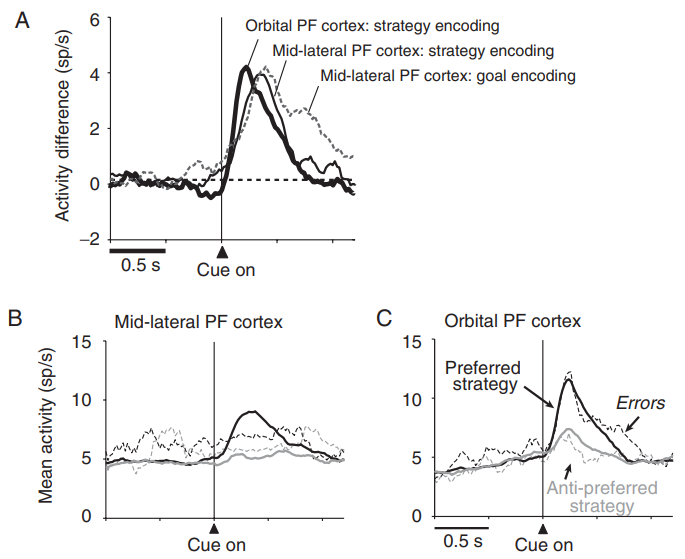
\includegraphics[width=0.5\linewidth]{image_pfc/Fig_6_15}
	\caption{中外侧和眶前皮层策略信号的时序。(A)来自眶部和中外侧前额皮质细胞群的策略编码信号,以及来自中外侧前额皮质细胞群的目标信号。(B)中外侧前部皮层正确与错误试验的活动。实线:正确试验的平均活动;虚线:错误试验的平均活动。黑线:首选策略;灰线,替代(反首选)策略。用虚线描述的活动在首选策略和反首选策略之间没有显著差异。(C)眶前皮层正确与错误试验的活动,见(B)。眶前皮层在正确和错误试验中有相同的策略信号。基于Tsujimoto S, genvesio A, Wise SP.背外侧和眶侧前额皮质策略信号的比较。Journal of Neuroscience, 31:4583-92,©Society for Neuroscience, 2011,已获授权}
	\label{fig:fig}
\end{figure}

图6.15提供了这类交互的一个示例。Tsujimoto等(2011a)研究了编码抽象策略的神经信号与编码抽象策略的神经信号之间的关系对基于这些策略选择的目标进行编码。第3章解释了这个任务,我们在本章的前面也提到过:一个有方向的条或一个彩色的方块提示猴子要么保持之前的目标,要么离开它。注视点左右的白色方块作为潜在目标。

Tsujimoto等人发现,眶前皮层的细胞比中外侧前皮层的细胞更早地编码该策略(图6.15A),这与OFC与下颞叶皮层的连接一致。当策略信号在中外侧前额皮质发育时,目标信号也出现在那里,这是OFC没有的特性。

中外侧和眶前部皮层在另一个方面也有所不同。在错误试验中,中外侧前部皮层的策略编码细胞显示出微弱的信号,如果有的话(图6.15B)。但是OFC中的细胞在错误试验中确实编码了正确的策略(图6.15C)。综上所述,这些结果表明,OFC向背侧PF皮层提供策略信号,在正确的实验中,后者根据该策略和记忆产生当前目标之前的目标。之后,不管选择是否正确,眶前皮层的其他细胞都会在反馈时对选择的目标进行编码。

除了表6.1中来自前部皮层背侧的连词编码的例子外,表8.2中还出现了其他连词编码的例子,我们将前部皮层视为一个整体。

\subsection{总结}
由于其与后顶叶皮层的连接,文献倾向于强调中外侧前部皮层在处理空间位置信息中的作用。然而,后顶叶细胞也编码时间间隔、时间和空间顺序、数量、大小、速度、长度和距离等信息。因此,它与后顶叶皮层的连接使中外侧前部皮层除了对事件的位置进行编码外,还能对事件的许多特征进行编码。中外侧前部皮层通过其顶叶和其他连接,对一系列先前选择的连词及其结果、顺序连词和相对持续时间、顺序连词和相对距离进行编码。

\section{结论}
\subsection{背侧前额皮质是如何工作的}
本章解释了背侧前部皮层的功能,一般来说,特别是中外侧前部皮层的功能,是如何依赖于它们的连接的:
\par
1.中外侧前部皮层与后顶叶皮层的连接不仅提供了视觉事件的位置信息,还提供了它们的持续时间和顺序,以及其他指标,如数量和相对距离。

这些联系解释了为什么延迟反应任务,以及其他类似的任务,主要依赖于中外侧前部皮层。给定一系列的试验,合适的目标取决于最近的视觉事件的位置,这决定了合适的当前目标。这种解释也解释了n-back任务的结果。例如,在“三回”任务中,正确的选择取决于三个事件之前出现在一系列事件中的项目。因此,我们认为后顶叶皮层向中外侧前部皮层提供的顺序信息在延迟反应任务等任务中起着关键作用。

由于其后顶叶连接,中外侧前部皮层位于背侧视觉流的末端,这一系统在行为的选择和控制中起着关键作用。持续的活动发生在整个系统的延迟期,例如在运动前皮层(Wise 1985), preSMA和SMA (Shima \& Tanji 2000),以及后顶叶皮层(Kalaska \& Crammon 1995)。延迟期活动和激活也发生在中外侧前部皮层。虽然我们知道中外侧前部皮层的许多细胞编码回溯性空间记忆(Genovesio等人,2006年b),并且它们在反扫视实验中编码提示位置(Funahashi等人,1993年3b),但成像结果显示,该区域的前瞻性编码激活比回溯性编码激活更占优势。
\par
2.中外侧前部皮层与OFC有紧密的连接(Barbas \& Pandya 1989),因此能够获取与当前需求相关的结果信息。
\par
3.通过与运动前区的连接,背侧前部皮层可以促进目标的实现。这些连接进入了专门控制手和手臂运动的前运动区域,而不是脚和腿的运动。这种专门化表明,背侧前部皮层产生的目标主要是为了达到运动和操纵。
\par
4.我们还提出,背侧前部皮层产生一系列有序的目标,这是计划一个序列所必需的,并且它与运动前区域的连接使顺序目标的实现成为可能。为了支持这一观点,preSMA中的一些细胞在一个序列中编码动作的等级顺序(Shima \& Tanji 2000),而其他细胞在猴子等待启动第一个动作时编码第二个动作(Nakajima et al 2009)。
\par
5.中外侧前部皮层(46区)和背内侧前部皮层(9区)的许多细胞编码顺序、持续时间、颜色、形状和结果等特征之间的连接,并且来自后顶叶皮层、眶和腹侧前部皮层、preSMA、周围皮层和其他区域的输入提供了大部分这些信息。我们在第8章中认为,这种高水平的整合源于PF皮层位于三个处理层次的顶端,一个处理背景,另一个处理目标,另一个处理结果。

由于延迟反应任务在文献中的重要性,本章强调延迟反应任务。早在75年前,Jacobsen就发现,有前脑皮层损伤的猴子(Jacobsen 1936)和黑猩猩(Jacobsen 1935)在这类任务中受到严重损害。20世纪80年代,Goldman-Rakic(1987)提出了PF皮层的工作记忆理论,这在很大程度上是基于延迟反应任务和相关任务的结果。她认为中外侧前部皮层(46区)在回溯性空间工作记忆中起着必要和特殊的作用(Goldman-Rakic 1998)。第10章对这一理论进行了一般性的讨论,在这里我们集中讨论它的联系方面。

与当时流行的关于背流和腹流功能的观点一致(Ungerleider \& Mishkin 1982), Goldman-Rakic强调了后顶叶皮层向前皮层提供的空间输入(Wilson etal 1993)。我们也强调这些连接的重要性,但对于它们为前皮层提供了什么,我们的解释不同。我们认为后顶叶皮层在视觉引导行为的选择和控制中起作用(Shadmehr \& Wise 2005;Milner \& Goodale 2007)。这一观点改变了我们对后顶叶皮层向中外侧前部皮层提供什么的理解(Rushworth 2000)。例如,当人们记住字母或形状时,那里就会发生成像激活(Rushworth \& Owen 1998)。人们可能会试图将它们纳入工作记忆理论,将中外侧前部皮层的作用扩展到非空间和空间工作记忆中。但更重要的因素是,这些激活发生在n -back任务中,这需要受试者记住项目出现的顺序(Nystrom et al . 2000)。所以这些观察确实表明,中外侧前部皮层的功能超越了空间分析,但它们可能反映了编码顺序的需要,而不是与工作记忆本身有关。

\subsection{提议}
我们现在可以提出一个关于前部皮层背侧功能的建议,附带条件是它主要集中在前部皮层中外侧(46区)。它以一种简短而又有些扩展的形式出现:

简而言之:

背侧前部皮层生成适合当前情境和期望结果的目标,其中最近发生的事件指定了该情境,并且它对这些目标进行前瞻性编码,直到可以尝试实现它们。

展开的:

背侧前部皮层根据当前环境生成目标,这些环境包括最近发生的事件,尤其是视觉事件的位置、持续时间、距离、数量、大小、速度和顺序。它利用这些特征,如空间和时间顺序,来产生具体和抽象的目标,以及这些目标的序列。必要时,它会前瞻性地对这些目标进行编码,直到可以尝试实现它们,并以这种方式击败来自不相关事件的干扰。

\subsection{为什么其他区域不能完成背侧前部皮层的功能}
我们认为后顶叶皮层为中外侧前部皮层提供了关键的输入。但如果这就是问题的全部,那么后顶叶皮层的损伤应该和中外侧前部皮层的损伤有同样的效果。很长一段时间以来,人们都知道它们不会。正如第一章所提到的,后顶叶皮层的损伤不会导致延迟反应(Alexander \& Fuster 1973)或延迟交替(Ettlinger etal 1966)任务的损害。作为这些发现的一个结果,我们可以得出结论,后顶叶皮层的细胞具有延迟期活动(Kalaska \& Crammond, 1995;Snyder等人2000)在这些任务中没有发挥必要的作用。

考虑到细胞活动提供的指导很少,我们转向解剖学来理解为什么中外侧前部皮层在延迟反应任务和相关任务中发挥必要的作用,而后顶叶皮层则没有。我们认为它们之间联系的差异可以解释这些发现。例如,后顶叶皮层缺乏中外侧前部皮层从眶前部皮层接收到的特定结果信息。第4章解释了关于特定结果的信息首先到达颗粒OFC,以颜色,形状和纹理视觉为主导。通过前皮层的内在联系,它可以很快到达中外侧前皮层,在那里它与有关目标的信息结合在一起。因此,中外侧前部皮层接收有关事件顺序的证据,以及与潜在目标及其当前价值相关的结果。后顶叶皮层有但只有中外侧前部皮层拥有基于当前情境和预测结果产生目标所需的所有信息。

\subsection{对觅食选择的贡献}
第2章解释了在类人猿灵长类动物的进化过程中出现了背侧前部皮层(参见Preuss 2011)。如果是这样,那么我们需要了解它带来了什么好处。关键可能在于基于视觉的觅食策略。早些时候,我们回顾了25门搜索任务的证据,该任务表明,中外侧和后外侧前部皮层受损的猴子以一种无序的方式搜索看不见的花生(Passingham 1985)。正常的猴子会按照有序的顺序搜索它们是否能看到目标(Desrochers et al . 2010) (Taffe \& Taffe 2011)。因此,背部前部皮层受损的猴子觅食效率似乎低于正常猴子。25扇门搜索任务需要“双赢”策略,延迟交替任务也是如此。一个优化的序列允许正常的猴子有效地实施这一策略。

当然,所有的动物都需要优化觅食,当第一个斑块耗尽时,从一个斑块移动到另一个斑块(Plank \& James 2008)。但这项25扇门的搜索任务并不需要通过移动从一个地方移动到另一个地方。类人猿优化觅食的方式强调达到目标,特别是在视觉事件的基础上这样做。高效的动作序列的优势可能与个体在群体觅食时面临的竞争有关。本章涉及中外侧前部皮层在使用视觉事件选择目标和生成有效的目标序列中的作用。这似乎使类人猿灵长类动物能够知道最近发生的视觉事件,包括它们的顺序、时间和位置,告诉它们下一步该做什么、,之后该做什么。当然,同样的能力使它们能够在新事件发生时改变觅食计划。

第2章还提出了类人猿灵长类动物在面对严重的资源波动问题时进化出背侧前部皮层的观点。在野外,类人猿根据同一树种的个体之间的同步性、经过的时间和天气事件(如持续的高温)来预测食物的可用性。这些预测依赖于物体表征(例如树或水果)与事件的顺序和时间的结合。背侧前部皮层代表这些类型的连词,它在识别先前事件的顺序与当前目标的选择直接相关方面发挥着必要的作用,无论是通过顺序编码还是规则编码。事件的持续时间和顺序,以及事件之间的间隔、数量、位置和相对距离,也会影响目标序列的规划。

本章提出,类人猿前部皮层的一个新进化部分,即背侧前部皮层,在很大程度上由其与后顶叶皮层的连接提供的当前环境中产生目标。我们认为它的功能反映了一种对日间觅食的适应:通过使用顺序、时间和距离信息有效地规划当前和未来的目标。另一部分颗粒状前部皮层也同时出现:腹侧前部皮层。下一章探讨了它用来产生目标的各种环境,以及允许它这样做的联系。